\documentclass[11pt]{article}

% package
\usepackage{amsmath,amssymb,amsthm}
\usepackage{graphicx}
\usepackage{caption}
\usepackage{subcaption}

% margin
\addtolength{\evensidemargin}{-.5in}
\addtolength{\oddsidemargin}{-.5in}
\addtolength{\textwidth}{0.8in}
\addtolength{\textheight}{0.8in}
\addtolength{\topmargin}{-.4in}

% custom definitions
\newtheoremstyle{quest}{\topsep}{\topsep}{}{}{\bfseries}{}{ }{\thmname{#1}\thmnote{ #3}.}
\theoremstyle{quest}
\newtheorem*{definition}{Definition}
\newtheorem*{theorem}{Theorem}
\newtheorem*{question}{Question}
\newtheorem*{exercise}{Exercise}
\newtheorem*{challengeproblem}{Challenge Problem}
\newcommand{\name}{

%% put your name here, so we know who to give credit to %%
[Your Name Here]
}
\newcommand{\hw}{
%% and which homework assignment is it? put the correct number below        
1
}

\title{\vspace{-50pt}
\Huge \name
\\\vspace{20pt}
\huge POLSCI 514\hfill Problem Set \hw}
\author{}
\date{}
\pagestyle{myheadings}
\markright{\name\hfill Problem Set \hw\qquad\hfill}

%% If you want to define a new command, you can do it like this:
%% The followins is the useful commands for math and probability. 
\newcommand{\R}{\mathbb{R}}
\newcommand{\E}{\mathbb{E}}
\newcommand{\V}{\mathbb{V}}



\begin{document}
\maketitle

\begin{question}[1]
  Replicate the following figure placement in LaTeX 
\end{question}

\begin{figure}[h]
     \centering
     \begin{subfigure}{0.45\textwidth}
         \centering
         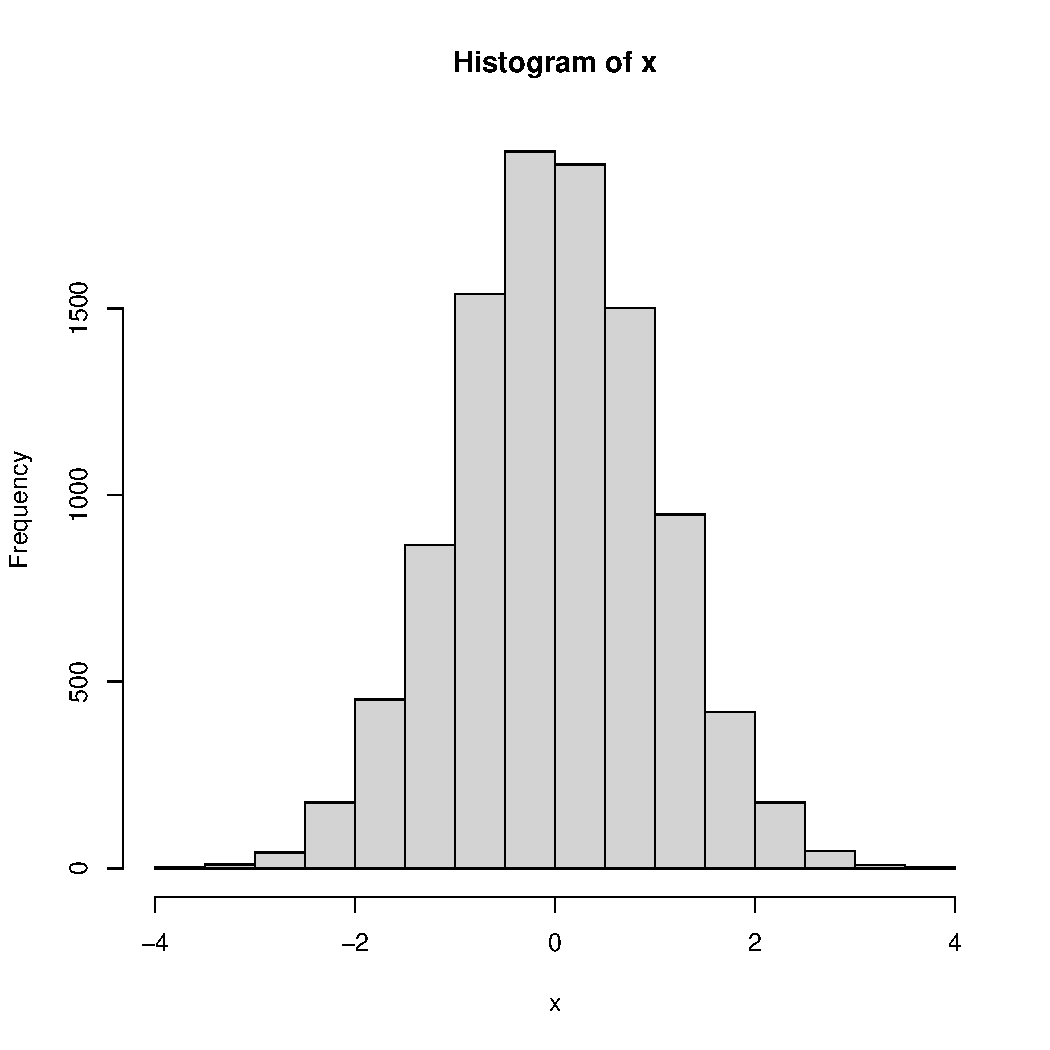
\includegraphics[width=\textwidth]{figs/normal.pdf}
         \caption{My first caption}
     \end{subfigure}
     \hfill
     \begin{subfigure}{0.45\textwidth}
         \centering
         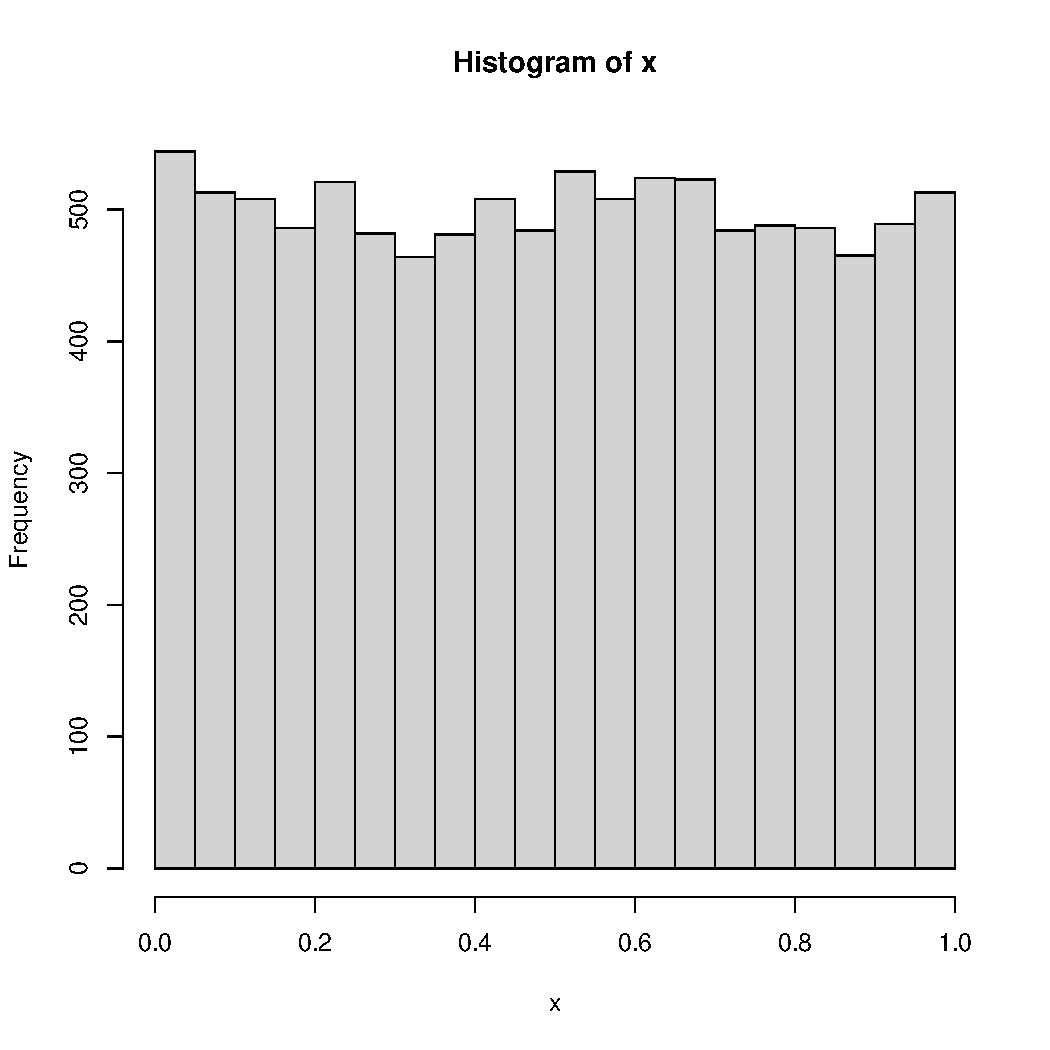
\includegraphics[width=\textwidth]{figs/unif.pdf}
         \caption{My second caption}
     \end{subfigure}
        \caption{Two distributions}
\end{figure}

\clearpage
\begin{question}[2]
  Replicate the following table placement in LaTeX 
\end{question}

\begin{table}[h!]
    \centering
    \begin{tabular}{|c||l|l|l|}
    \hline
    $x$ & 1 & 2 & 3\\
    \hline
    $f(x)$ & 4 & 8 & 12\\
    $g(x)$ & 1.5 & 3.0 & 4.5\\
    \hline
    \end{tabular}
    \caption{This is my first table.}
\end{table}

\begin{table}[h!] % start a float for a table
\centering
\begin{tabular}{ll|rr}
% NOTE: {l: left, r: right, c: center} will specify the location of text within a cell.
% |: vertical bar of the table
\hline
\hline
Category &  & 20XX Census & Survey Respondents \\ 
\hline
Gender & Male & 50.0\% & 51.0\% \\ 
   & Female & 48.5\% & 48.0\% \\ 
   & Other & 1.5\% & 1.0\% \\ 
\hline
Education & High School & 90.5\% & 91.2\%  \\ 
   & Bachelor's or Higher & 35.0\% & 40.0\% \\ 
\hline
\hline
\end{tabular}
\caption{Table of summary statistics about the respondents.}
\end{table}

%%%% don't delete the last line!
\end{document}
